%\documentclass{beamer}
\documentclass[handout,xcolor=pdftex,dvipsnames,table]{beamer} % for handouts

%\graphicspath{{/Users/niemi/desktopBackup/Users/niemi/research/presentations/2011/ABC/}}

\usecolortheme[RGB={0,0,144}]{structure}
\usetheme{AnnArbor}\usecolortheme{beaver}
%\usetheme{CambridgeUS}\usecolortheme{crane}

\usepackage{verbatim,xmpmulti,color,multicol,multirow}
\setlength{\unitlength}{\textwidth}  % measure in textwidths


%\usepackage{beamerthemesplit}
\setbeamertemplate{navigation symbols}{}
%\setbeamercolor{alerted text}{fg=red}
%\setbeamertemplate{block body theorem}{bg=orange}
\setkeys{Gin}{width=0.6\textwidth}


\newcommand{\curdate}{28 Sep 2011}
\newcommand{\lecturetitle}{Statistical computation on GPGPUs}

\title[CompStats on GPGPUs]{\lecturetitle}
\author{Jarad Niemi\\Matthew Wheeler}
\institute[Iowa State]{Iowa State University}
\date{\curdate}

\newcommand{\iid}{\stackrel{iid}{\sim}}
\newcommand{\Yiid}{Y_1,\ldots,Y_n\stackrel{iid}{\sim}}

\begin{document}

%\section{Temp??} \begin{comment}

\frame{\titlepage}

\section{Introduction}
\subsection{Outline}
\frame{\frametitle{Outline}
	\begin{itemize}
	\item Results
	\item Parallelism 
		\begin{itemize}
		\item General
		\item Statistics
			\begin{itemize}
			\item Optimization (MLEs)
			\item Integration (Posteriors)
			\end{itemize}
		\end{itemize}
	\item GPGPUs
		\begin{itemize}
		\item What?
		\item How?
		\end{itemize}
	\item An example - stochastic chemical kinetic models (skip?)
	\item Wrap-up
		\begin{itemize}
		\item Parallelism coming to the end user?
		\end{itemize}
	\end{itemize}
}


\section{Results}
\frame{\frametitle{}
	\begin{center}
	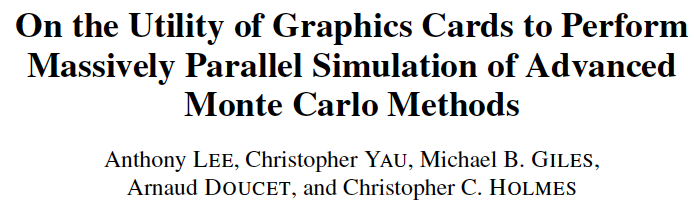
\includegraphics{Lee}
	\end{center}
	
	\vspace{0.2in}
	
	\begin{center}
	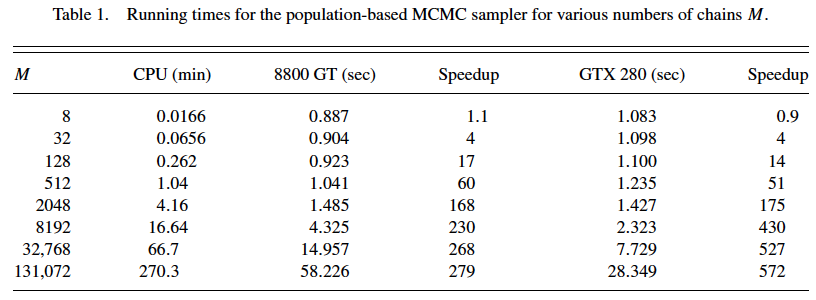
\includegraphics[width=4.5in]{Lee1}
	\end{center}
}\frame{\frametitle{}
	\begin{center}
	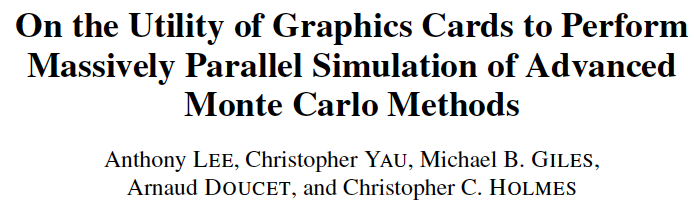
\includegraphics{Lee}
	\end{center}
	
	\vspace{0.2in}
	
	\begin{center}
	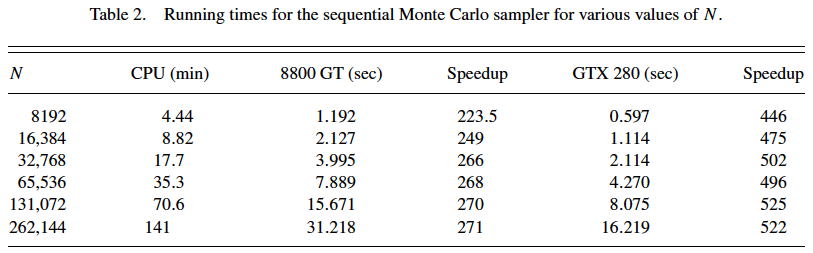
\includegraphics[width=4.5in]{Lee2}
	\end{center}
}\frame{\frametitle{}
	\begin{center}
	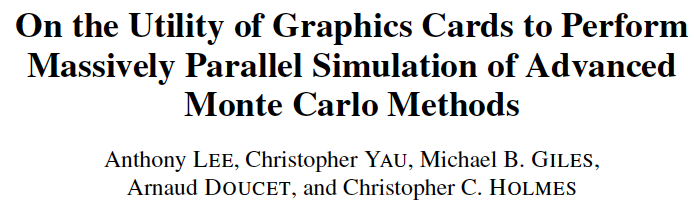
\includegraphics{Lee}
	\end{center}
	
	\vspace{0.2in}
	
	\begin{center}
	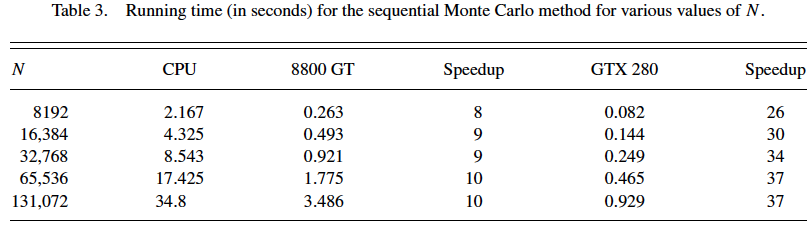
\includegraphics[width=4.5in]{Lee3}
	\end{center}
}

\frame{\frametitle{}
	\begin{center}
	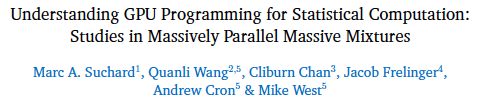
\includegraphics{Suchard}
	\end{center}
	\begin{table}
	{\scriptsize
	\begin{tabular}{l|r@{.}lr@{.}lr@{.}lrr|r@{.}lr}
	n & \multicolumn{2}{c}{gpu 1} & \multicolumn{2}{c}{gpu 3} & \multicolumn{2}{c}{tesla} & \multicolumn{1}{c}{cpu 8} & \multicolumn{1}{c|}{cpu 1} & \multicolumn{2}{c}{mac gpu} & \multicolumn{1}{c}{mac cpu} \\
	\hline
	$10^2$ & 1&225 & 1&243 & 1&226 & 3.0 & 3.0 & 2&119 & 5.0 \\
	$10^3$ & 1&42 & 1&36 & 1&45 & 20.0 & 20.0 & 3&654 & 30.0 \\
	$10^4$ & 3&18 & 2&46 & 3&49 & 94.0 & 191.0 & 18&78 & 277.0 \\
	$10^5$ & 20&4 & 13&1 & 23&7 & 386.0 & 1,907.0 & 169&7 & 2,758.0 \\
	$10^6$ & 192&0 & 119&5 & 224&6 & 3,797.0 & 19,048.0 & 1,118&1 &
27,529.0 \\
	$5\times 10^6$ & 954&0 & 591&0 & 1,116&0 & 17,667.0 & 95,283.0 & 5,785&8 & 141,191.0 \\
	\hline
	\end{tabular}
	\vspace{0.2in}
	
	\caption{Running times (in seconds) for 100 iterations of the MCMC analysis of TDP model}
	}
	\end{table}
}


\subsection{Rejection sampling}
\frame{\frametitle{}
	\begin{center}
	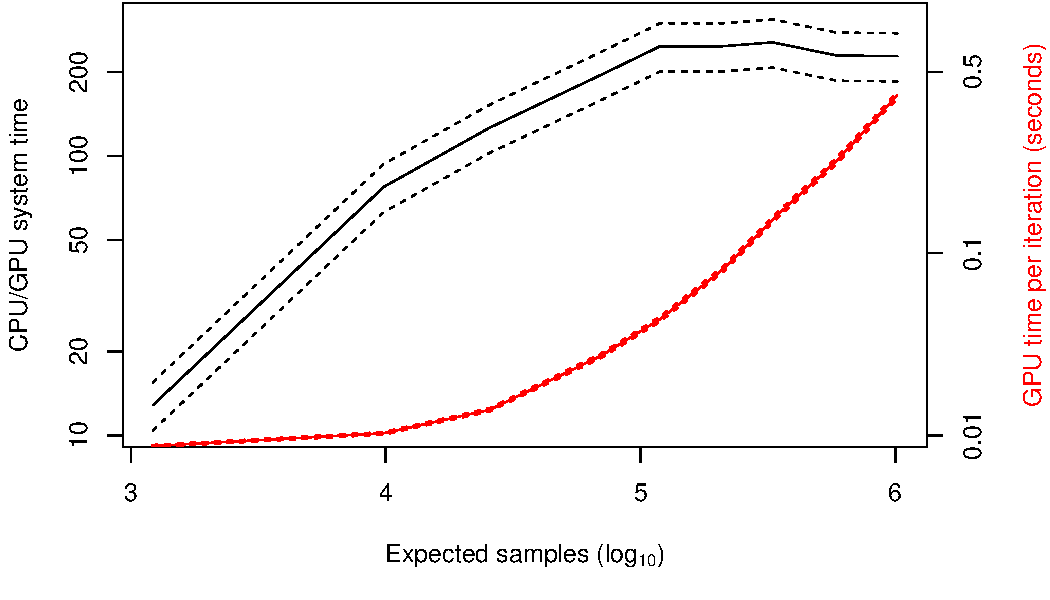
\includegraphics[width=4.5in]{Michaelis-Menton-CPUvsGPU}
	\end{center}
}


\subsection{Spatial statistics}
\frame{\frametitle{}
	\begin{center}
	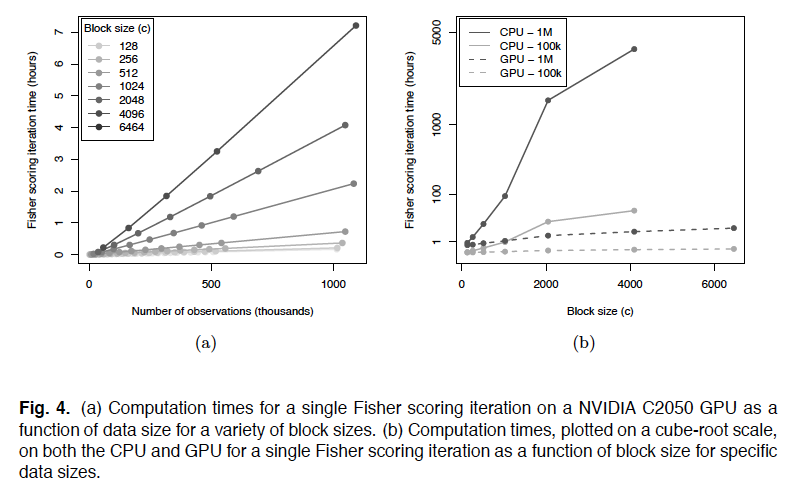
\includegraphics[width=4.5in]{FisherScoring}
	\end{center}
	The speedup was 1.4-fold at c = 128, 13-fold at c = 512, 29-fold at c = 1024, and 112-fold at c = 4096.
}

\section{Parallelism}
\subsection{Amdahl's quantity}
\frame{\frametitle{}
	Theoretical maximum speedup, Amdahl's quantity:
		\[ \frac{1}{1-P+\frac{P}{N}} \]
	\begin{itemize}
	\item[] $P$: fraction of the program that can be parallelized
	\item[] $N$: number of parallel processors
	\end{itemize}
	
	\vspace{0.2in} \pause
	
	As $N\to\infty$:
		\[ \frac{1}{1-P} \]
	
	\vspace{0.2in} \pause
	
	So if 99\% of the program can be parallelized, theoretically we could have a 100-fold speedup.
}

\subsection{What's N?}
\frame{\frametitle{What's N?}\pause
	\begin{itemize}
	\item CPU
		\begin{itemize}
		\item Clusters: multiple CPUs/memory networked \pause (CyBlue: N=1-2k) \pause
		\item Multicores: 2-6 CPUs with shared memory \pause (N=2-6) \pause
		\end{itemize}
	\item GPU
		\begin{itemize}
		\item Single card: many-core with own, shared memory attached to CPU \pause (N=448) \pause
		\item Cluster: multiple GPUs with CPU(s) \pause (N=4x448) 
		\end{itemize}
	\end{itemize}
	
	\vspace{0.1in} \pause
	
	\begin{center}
	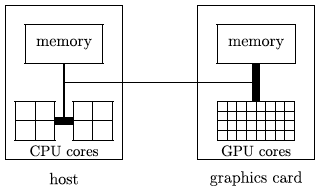
\includegraphics[width=2in]{Lee4}
	
	{\tiny From Lee et. al.}
	\end{center}
	\pause
	FLOPS, a measure of performance: CyBlue: 5.7TF, Tesla C2050: 1.0TF
}

\subsection{What's P?}
\frame{\frametitle{What's P?}
	Flynn's taxonomy
	\begin{center}
	\begin{tabular}{r|rr}
	& Single instruction & Multiple instruction \\
	\hline 
	Single data & SISD & MISD \\
	Multiple data & SIMD & MIMD 
	\end{tabular}
	\end{center}
	
	\vspace{0.2in} \pause
	
	\begin{itemize}
	\item SISD: no parallelism \pause
	\item SIMD: good for CPU/GPU parallelism \pause
	\item MISD: fault tolerance, e.g. Space Shuttle flight controller \pause
	\item MIMD: possible for CPU/GPU parallelism (edge to CPUs)
	\end{itemize}
	
	\vspace{0.2in}\pause
	
	{\tiny From Wikipedia: \url{http://en.wikipedia.org/wiki/Flynn's_taxonomy}}
}

\frame{\frametitle{Multiplying matrices}
	Let 
	\[ 
	A = \left[ \begin{array}{cc} a_{11} & a_{12} \\ a_{21} & a_{22} \end{array} \right], \qquad
	B = \left[ \begin{array}{cc} b_{11} & b_{12} \\ b_{21} & b_{22} \end{array} \right]
	\]
	and you are interested in $C=AB$. 
	
	\vspace{0.2in} \pause
	
	\begin{columns}[t]
	\begin{column}{0.5\textwidth}
	The \alt<1-5>{SISD calculation}{\alert{SIMD threads}}:
	\begin{enumerate}[1.]
	\item $c_{11} = a_{11}b_{11}+a_{12}b_{21}$ \pause
	\item $c_{12} = a_{11}b_{12}+a_{12}b_{22}$ \pause
	\item $c_{21} = a_{21}b_{11}+a_{22}b_{21}$ \pause
	\item $c_{22} = a_{21}b_{12}+a_{22}b_{22}$ \pause\pause
	\end{enumerate}
	\end{column}
	\begin{column}{0.5\textwidth}
	What's P?
	
	\vspace{0.1in} \pause
	
	If square matrices of size $n$, \pause then \\
	repeat $n^2$-times \pause
	\begin{itemize}
	\item $n$ products\pause
	\item $n-1$ sums\pause
	\end{itemize}
	Intuitively, as $n\to\infty$ then $P\to1$.
	\end{column}
	\end{columns}
}

\subsection{Statistics}
\frame{\frametitle{Parallel tempering}
	\begin{itemize}
	\item Run $M$ \alert{independent} MCMC chains at various temperatures, i.e. flattenings of the likelihood. \pause
	\item At the end of each MCMC iteration, swap states in adjacent chains with the appropriate probability. \pause 
	\item Only take samples from the unflattened chain.
	\end{itemize}
	
	\vspace{0.2in} \pause
	
	As $M\to\infty$, $P\to1$.
}

\frame{\frametitle{Sequential Monte Carlo}
	\begin{itemize}
	\item Have $N$ weighted particles, approximating a posterior distribution.
	\item After collecting new data, each particle updates \alert{independently}.
	\item Particles are reweighted.
	\end{itemize}
	
	\vspace{0.2in} \pause
	
	As $N\to\infty$, $P\to1$.
}

\frame{\frametitle{Latent variable modeling}
	\begin{itemize}
	\item Each observation has an associated latent variable. 
	\item One step in the MCMC is to \alert{independently} update each observations latent variable.
	\end{itemize}
	
	\vspace{0.2in} \pause
	
	As data size $\to\infty$, $P\to1$.
}

\frame{\frametitle{Rejection sampling}
	\begin{itemize}
	\item Attempting to sample from $p(\cdot)$.
	\item Sample $x\sim q(\cdot)$, accept with probability $p(x)/Mq(x)$. 
	\end{itemize}
	
	\vspace{0.2in} \pause
	
	As $p(x)/Mq(x)\to 0$, $P\to1$.
}

\frame{\frametitle{Spatial analysis}
	\begin{itemize}
	\item Split data (size $n$) into blocks of size $c$ \pause
	\item Calculate inverses and determinants of pairwise block covariances
	\end{itemize}
	
	\vspace{0.2in} \pause
	
	Two opportunities for parallelization: \pause
	\begin{itemize}
	\item $c\to\infty,n\to\infty, \implies P\to1$, \pause but cannot load into memory! \pause
	\item $c\to 0,n\to\infty, \implies$ number of pairwise comparisons $\to\infty$, $P\to1$.
	\end{itemize}
	
	\vspace{0.2in} \pause
	
	Since blocks are an approximation, choose largest possible $c$ and use GPU to calculate inverses and determinants. 
}

\subsection{Summary}
\frame{\frametitle{}
\begin{itemize}[<+->]
\item	Lots of opportunity for parallelism
	\begin{itemize}
	\item data size increases
	\item approximating samples increases
	\item number of chains increases \\
	(very large?, suitable for CPU parallelization)
	\end{itemize}
	
	\vspace{0.2in} 
	
\item	Reduced computing time is on the order of 200
	\begin{itemize}
	\item 6 months becomes 1 day
	\item 1 day becomes 7 minutes
	\item 1 minute becomes a fraction of a second
	\end{itemize}
\end{itemize}
}


\section{GPGPUs}
\subsection{What?}
\frame{\frametitle{}
\setkeys{Gin}{width=\textwidth}
General purpose graphical processing units (GPGPUs)
	\begin{columns}[t]
	\begin{column}{0.5\textwidth}
	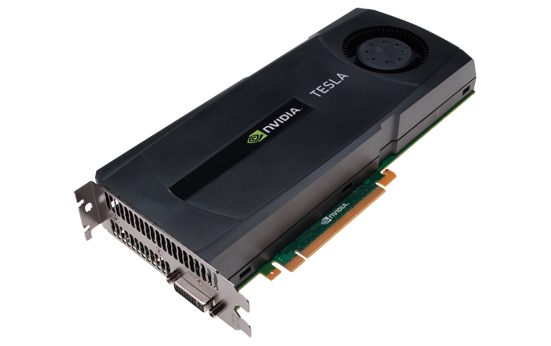
\includegraphics{Nvidia_Tesla_C2050_C2070}
	
	NVIDIA Tesla C2075 \\
	Ebay: \$1750 \\
	Cores: 448 \\
	Memory: 6GB \\
	* Higher fault tolerance * \\
	\end{column}
	\begin{column}{0.5\textwidth}
	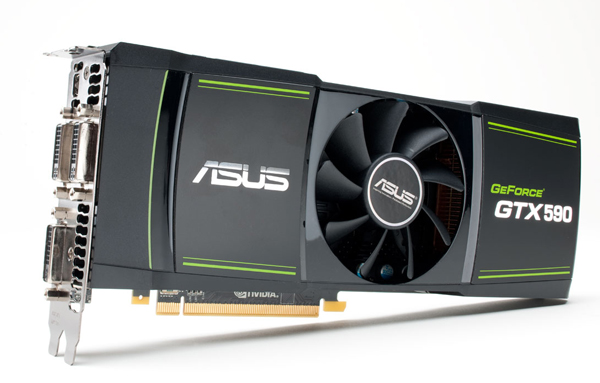
\includegraphics{vidcard_gtx590_7197}
	
	NVIDIA GeForce GTX 590 \\
	Ebay: \$840 \\
	Cores: 1024 \\
	Memory: 3GB \\
	* No faults detected * \\
	\end{column}
	\end{columns}
	
	\vspace{0.2in} 
	
	\begin{center}
	** Require PCI-E 2.0 x16 bus ** 
	\end{center}
}

\subsection{How?}
\frame[containsverbatim]{\frametitle{Coding in C}	
	\begin{verbatim}
	#include <iostream>
	
	int main ( void ) {
	  printf( "Hello, World!\n" );
	  return 0;
	}
	\end{verbatim}
}

\frame[containsverbatim]{\frametitle{Coding in CUDA C}	
	\begin{verbatim}
	#include <iostream>
	
	__global__ void kernel ( void ) {
	}
	
	int main ( void ) {
	  kernel<<<1,1>>>();
	  printf( "Hello, World!\n" );
	  return 0;
	}
	\end{verbatim}
}

\frame[containsverbatim]{\frametitle{}	\tiny
	\begin{verbatim}
#include "../common/book.h"

# define N 10

int main( void ) {
  int a[N], b[N], c[N];
  int *dev_a, *dev_b, *dev_c;
  
  // allocate memory on the GPU
  HANDLE_ERROR( cudaMalloc( (void**)&dev_a, N * sizeof(int) ) );
  HANDLE_ERROR( cudaMalloc( (void**)&dev_b, N * sizeof(int) ) );
  HANDLE_ERROR( cudaMalloc( (void**)&dev_c, N * sizeof(int) ) );
  
  // fill the arrays 'a' and 'b' on the CPU
  for (int i=0; i<N; i++) {
    a[i] = -i;
    b[i] = i * i;
  }
  
  // copy the arrays 'a' and 'b' to the GPU
  HANDLE_ERROR( cudaMemcpy( dev_a, a, N * sizeof(int), cudaMemcpyHostToDevice ) );
  HANDLE_ERROR( cudaMemcpy( dev_b, b, N * sizeof(int), cudaMemcpyHostToDevice ) );
  
  add<<<N,1>>>( dev_a, dev_b, dev_c);
  
  // copy array 'c' back from the GPU to the CPU
  HANDLE_ERROR( cudaMemcpy( c, dev_c, N * sizeof(int), cudaMemcpyDeviceToHost ) );
  
  // display the results
  for (int i=0; i<N; i++) { printf( "%d + %d = %d\n", a[i], b[i], c[i] ); }
  
  // free memory allocated on the GPU
  cudaFree( dev_a );
  cudaFree( dev_b );
  cudaFree( dev_c );
	\end{verbatim}
}

\frame[containsverbatim]{\frametitle{Coding in CUDA C}	

The GPU kernel:

\vspace{0.2in}
{\small
	\begin{verbatim}
__global__ void add( int *a, int *b, int *c ) {
  int tid = blockIdx.x;     // handle the data at this index
  if (tid < N)
    c[tid] = a[tid] + b[tid];
}
	\end{verbatim}
	}
}
	
\frame[containsverbatim]{\frametitle{Coding in CUDA C}	
SIMD: each block acts on its own data

\vspace{0.2in}

The code each block ``sees'':

\vspace{0.1in}
	
{\small
	Block 1
	\begin{verbatim}
__global__ void add( int *a, int *b, int *c ) {
  int tid = 0;     // handle the data at this index
  if (tid < N)
    c[tid] = a[tid] + b[tid];
}
	\end{verbatim}
}

{\small	
	Block 2
	\begin{verbatim}
__global__ void add( int *a, int *b, int *c ) {
  int tid = 1;     // handle the data at this index
  if (tid < N)
    c[tid] = a[tid] + b[tid];
}
	\end{verbatim}
}
}

\frame{\frametitle{}
\setkeys{Gin}{width=0.5\textwidth}
	\begin{center}
	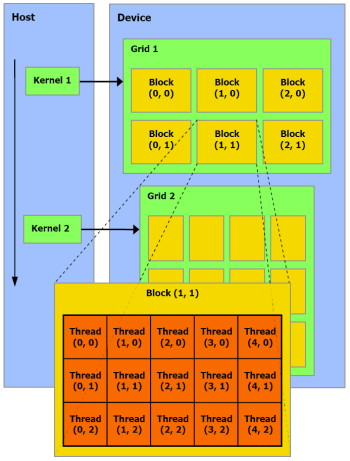
\includegraphics{IMG0020712}
	\end{center}
}

\frame{\frametitle{}
\setkeys{Gin}{width=0.6\textwidth}
	\begin{center}
	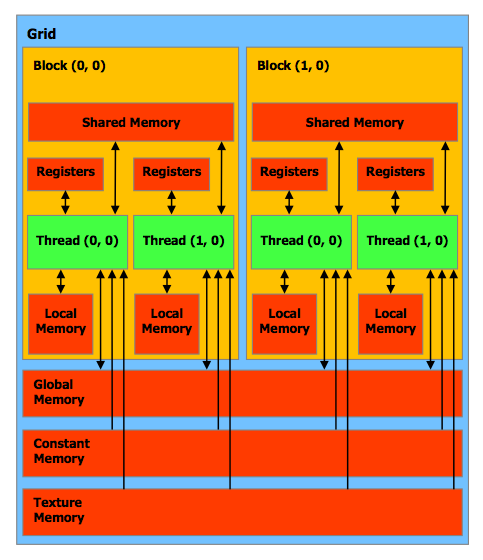
\includegraphics{screenshot_316}
	\end{center}
}

\frame{\frametitle{}
{\tiny
\begin{tabular}{lrl}
Device 0: "Tesla T10 Processor" \\
 CUDA Driver Version:                   &        3.10 \\
 CUDA Runtime Version:                  &        3.10 \\
 CUDA Capability Major revision number: &        1 \\
 CUDA Capability Minor revision number:   &      3 \\
 Total amount of global memory:               &  4294770688 & bytes \\
 Number of multiprocessors:                   &  30 \\
 Number of cores:                              & 240 \\
 Total amount of constant memory:      &         65536 & bytes \\
 Total amount of shared memory per block:   &    16384 & bytes  \\
 Total number of registers available per block: &16384 \\
 Warp size:                                    &  32 \\
 Maximum number of threads per block:          & 512 \\
 Maximum sizes of each dimension of a block:  &  512 x 512 x 64 \\
 Maximum sizes of each dimension of a grid:    & 65535 x 65535 x 1 \\
 Maximum memory pitch:                 &         2147483647 & bytes \\
 Texture alignment:                           &  256 &bytes \\
 Clock rate:                                    &1.44 &GHz \\
 Concurrent copy and execution:     &            Yes \\
 Run time limit on kernels:                  &   No \\
 Integrated:                                   & No \\
 Support host page-locked memory mapping: &      Yes \\
 Compute mode:                                &  \multicolumn{2}{l}{Default (multiple host threads can use this device simultaneously)} 
 \end{tabular}
 }
 
 \vspace{0.4in}\pause
 
 \hyperlink{wrapup}{Wrap-up}
}




\section{Stochastic chemical kinetic models}
\subsection{Terminology}
\frame{\frametitle{}
	\setkeys{Gin}{width=0.8\textwidth}
	Imagine a \emph{well-mixed} system in \emph{thermal equilibrium} with
	\begin{itemize}[<+->]
	\item $N$ species: $S_1,\ldots,S_N$ with
	\item number of molecules $X_1,\ldots,X_N$ with elements $X_j\in\mathbb{Z}^+$
	\item which change according to $M$ reactions: $R_1,\ldots,R_M$ with
	\item propensities $a_1(x),\ldots,a_M(x)$.  
	\item The propensities are given by $a_j(x) = \theta_j h_j(x)$ 
	\item where $h_j(x)$ is a known function of the system state. 
	\item If reaction $j$ occurs, the state is updated by the stoichiometry $\nu_j$ with 
	\item elements $\nu_{ij}\in\{-1,0,1\}$. 
	\end{itemize}
	
	\begin{columns}
	\hspace{0.15in}
	\begin{column}{0.8\textwidth}
	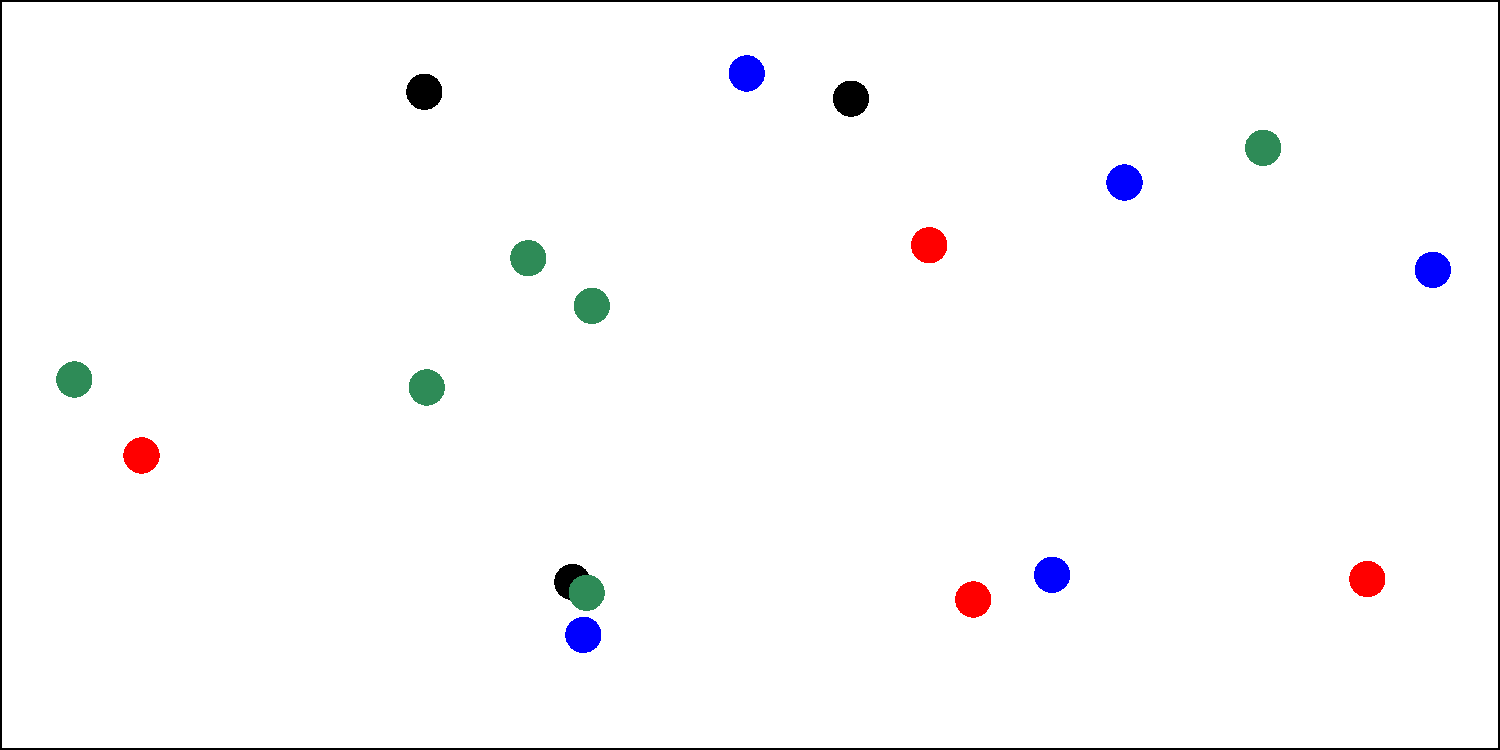
\includegraphics{system}
	\end{column}
	\hspace{-.6in}
	\begin{column}{0.4\textwidth}
	\uncover<3->{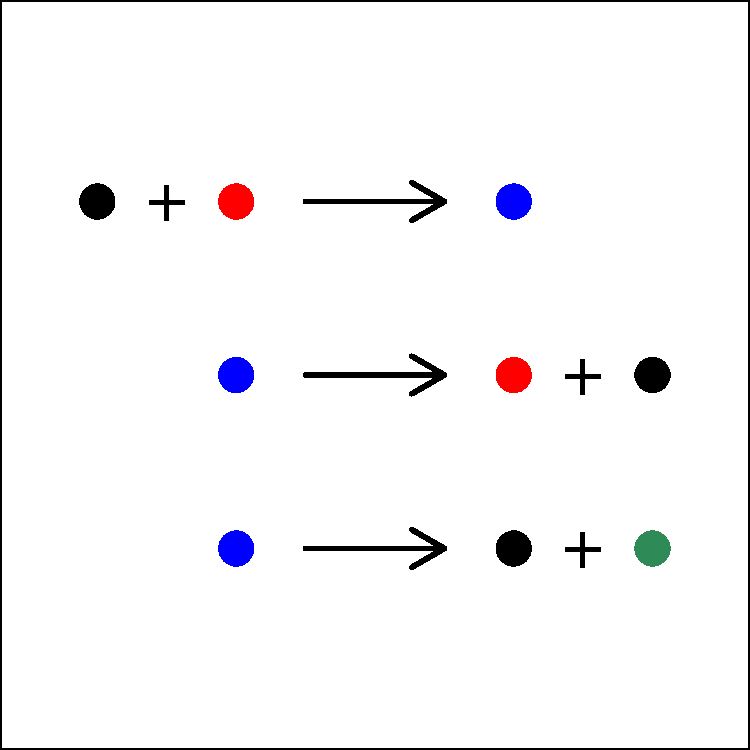
\includegraphics{rxns}}
	\end{column}
	\end{columns}
}

\subsection{Gillespie algorithm}
\frame{\frametitle{}
	\setkeys{Gin}{width=0.6\textwidth}
	{\small
	\begin{itemize}
	\item If reaction $j\in\{1,\ldots,M\}$ has the following probability
	\[ \lim_{dt\to 0} P(\mbox{reaction $j$ within the interval $(t,t+dt)$}|X_t) = a_j(X_t) dt,  \]
	\item[] then this defines a \alert{continuous-time Markov jump process}. \pause
	\item Then a realization from this model can be obtained using the Gillespie algorithm:
		\begin{itemize}
		\item For $j\in\{1,\ldots,M\}$, calculate $a_j(X_t)$.
		\item Calculate $a_0(X_t) = \sum_{j=1}^M a_j(X_t)$.
		\item Simulate a reaction time $\tau \sim Exp(a_0(X_t))$ 
		\item Simulate a reaction id $k\in\{1,\ldots,M\}$ with probability $a_k(X_t)/a_0(X_t)$
		\end{itemize}
	\end{itemize}
	}
	
	\vspace{0.05in} 
	
	\begin{center}
	\uncover<3->{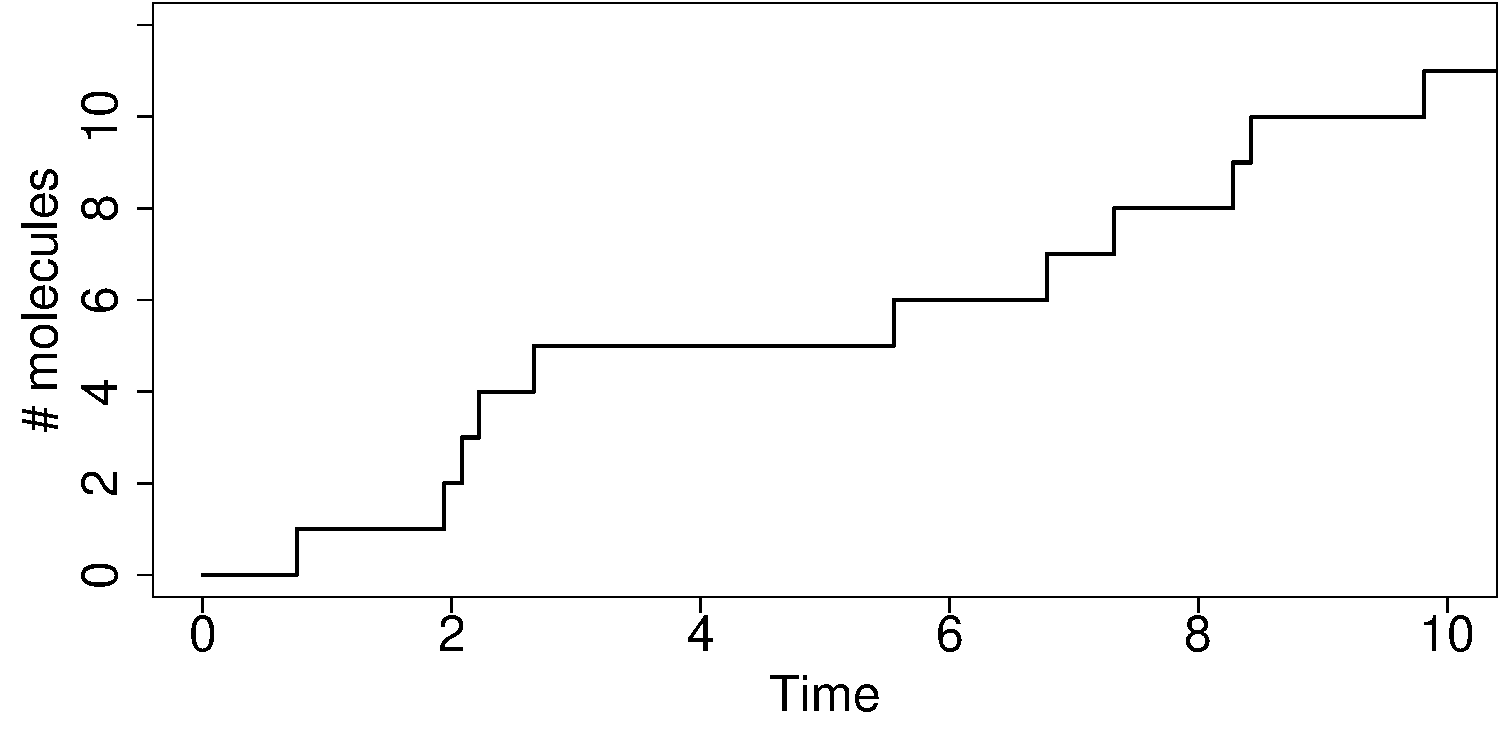
\includegraphics{production}}
	\end{center}
}

\subsection{Complete observations}
\frame{\frametitle{}
	Suppose you observe all system transitions:
	\begin{itemize}
	\item $n$ reactions occur in the interval $[0,T]$ 
	\item $t_1,\ldots,t_n$ are the reaction times 
	\item $r_1,\ldots,r_n$ are the reaction indicators, $r_i\in\{1,\ldots,M\}$
	\end{itemize}
	
	\vspace{0.2in} \pause
	
	Then inference can be performed based on the likelihood
	\[ 
	L(\theta) \propto \prod_{j=1}^M \theta_j^{n_j} \exp\left(-\theta_j I_j \right) 
	\]
	\pause where
	\[ \begin{array}{lll}
	n_j &= \sum_{i=1}^n \mathrm{I}(r_i=j) & \mbox{\# of $j$ reactions} \\ \\
	I_j &= \int_0^T h_j(X_t) dt &= \sum_{i=1}^n h_j(X_{t_{i-1}}) (t_i-t_{i-1}) + h_j(X_{t_n})[T- t_n]
	\end{array} \]
}

\subsection{Discrete observations}
\frame{\frametitle{}
	Suppose you only observe the system at discrete-times: 
	\begin{itemize}
	\item For simplicity, observe the system at times $t=1,2,\ldots,T$. 
	\item At these times, we observe $y_t=X_t$ the system state. 
	\item But do not observe the system between these times. \pause
	\end{itemize}
	\setkeys{Gin}{width=\textwidth}
	\begin{center}
	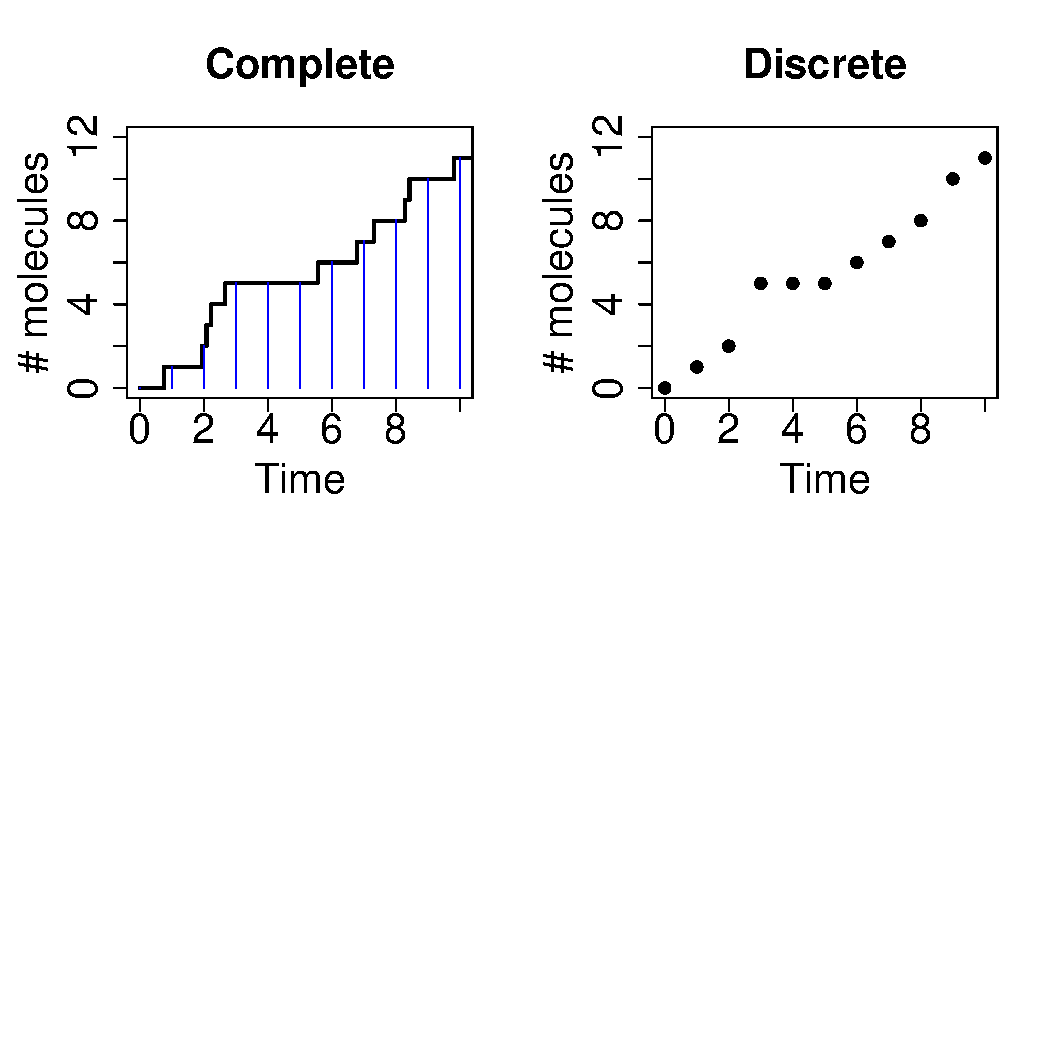
\includegraphics{discrete}
	\end{center}
}

\subsection{Inference}
\frame{\frametitle{}
	Inference is still performed based on the likelihood
	\[ L(\theta) = p(y|\theta) = p(t,y)  \]
	\pause but this is the solution to the \alert{chemical master equation}
	\[
	\frac{\partial}{\partial t}p(t,y) = \sum_{j=1}^M \big(a_j(y-\nu_m)p(t,y-\nu_m)- a_j(y)p(t,y)\big)
	\]
	which is generally intractable.
}

\subsection{Gibbs sampling}
\frame{\frametitle{Gibbs sampling}
	\setkeys{Gin}{width=\textwidth}
	Our objective is samples from the posterior 
	\[ p(\theta|y) \pause =\int p(\theta,X|y) dX \pause \propto \int p(y|X)p(X|\theta)p(\theta) dX \]
	\begin{columns}
	\begin{column}{0.6\textwidth}
	\pause A Gibbs sampling procedure is \pause
	\begin{enumerate}[1.]
	\item Start with $\theta^{(0)},X^{(0)}$ \pause
	\item For $k=1,\ldots,K$, 
		\begin{enumerate}[a.]
		\item Sample $X^{(k)}\sim p(X|\theta^{(k-1)},y)$ \\a.k.a. rejection sampling \pause
		\item Sample $\theta^{(k)}\sim p(\theta|X^{(k)})$ \pause
		\end{enumerate}
	\end{enumerate}
	
	\vspace{0.2in}
	
	$\theta^{(k)},X^{(k)}$ converge to samples from $p(\theta,X|y)$ \pause
	
	\end{column}
	\begin{column}{0.4\textwidth}
	\begin{center}
	\only<1-| handout:0>{\multiinclude[<+>][format=pdf]{gibbs}}
    \only<beamer:0| handout:1>{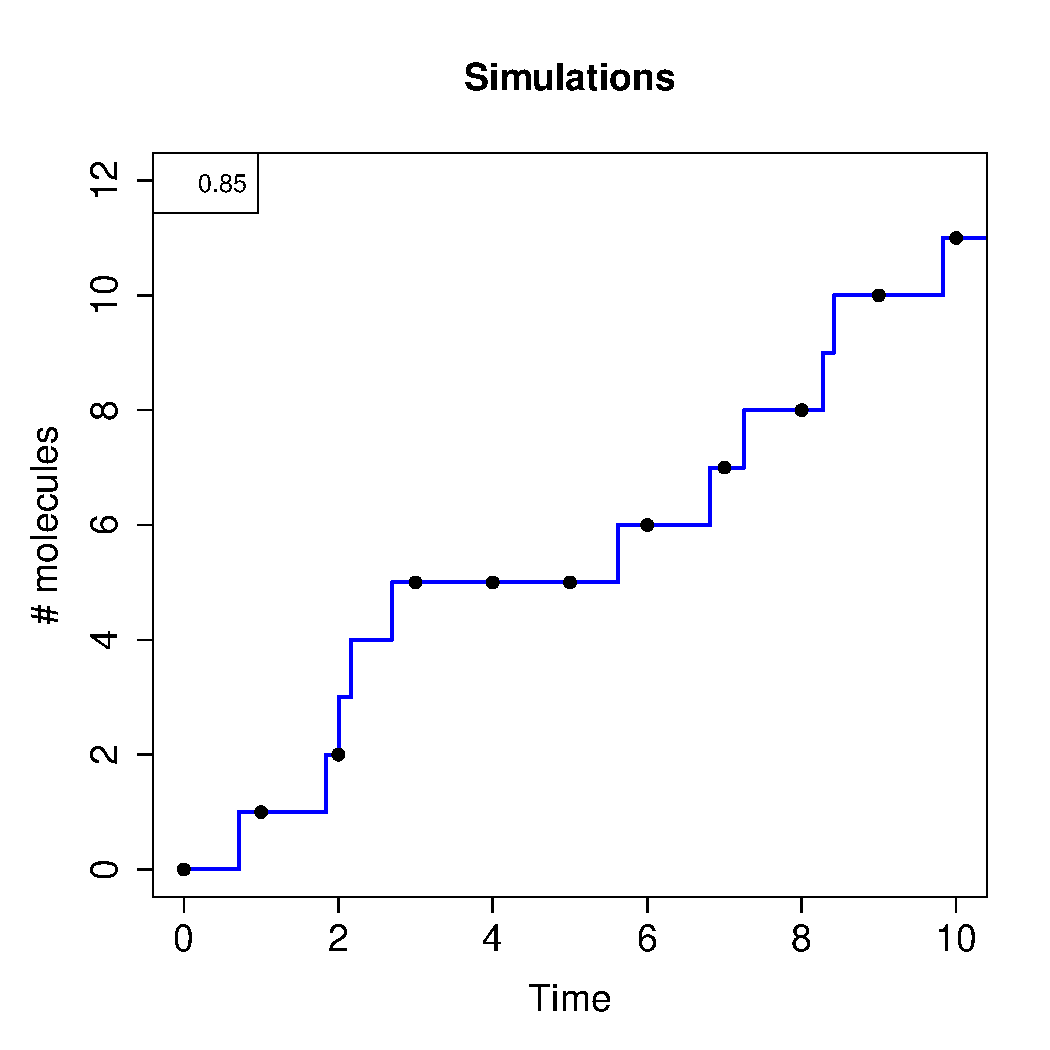
\includegraphics{gibbs-9}}
	\end{center}
	\end{column}
	\end{columns}
}

\subsection{Posteriors}
\frame{\frametitle{Posteriors}
	\setkeys{Gin}{width=\textwidth}
	\begin{center}
	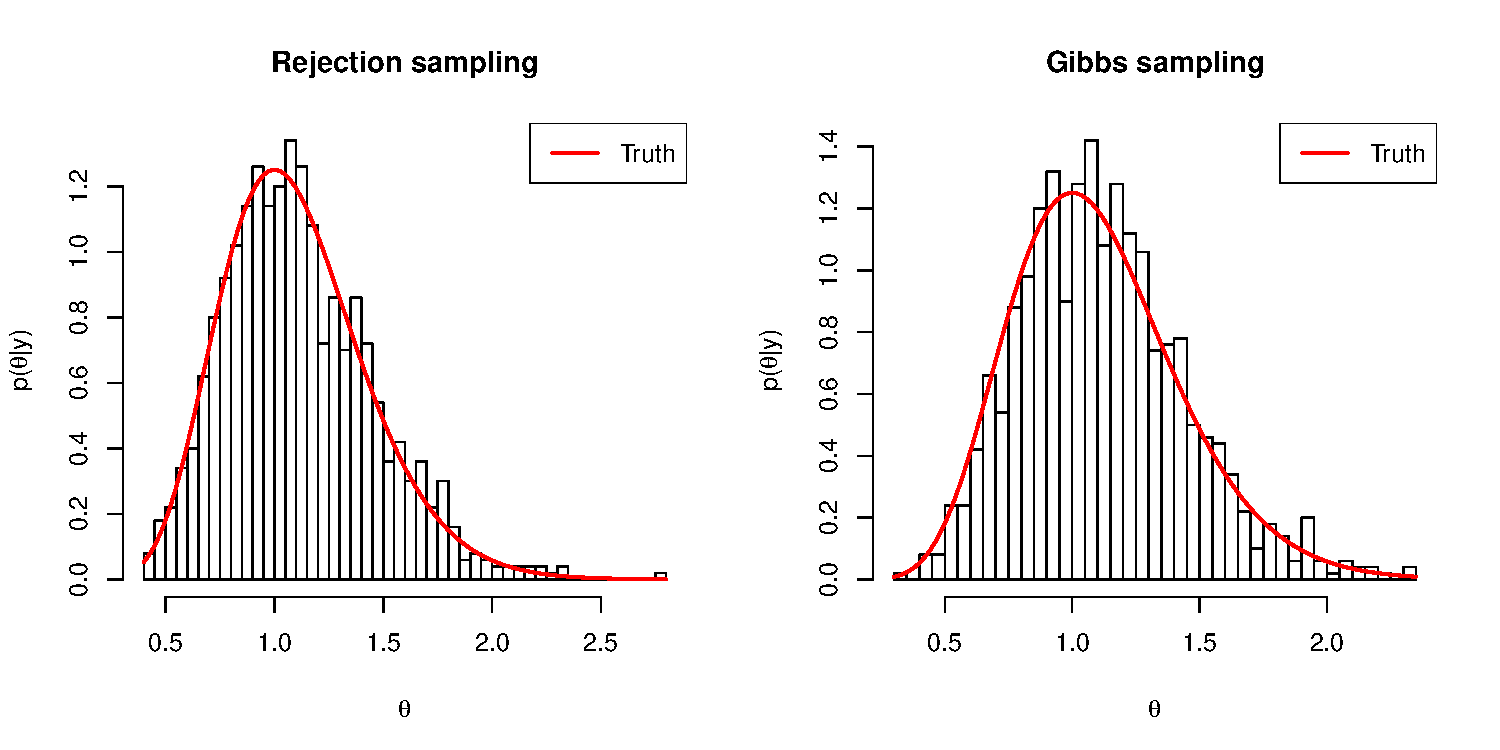
\includegraphics{posterior}
	\end{center}
	
	\pause \alert{So what's the problem?} \pause Extremely high rejection rates!!
}

\subsection{Modification to GPGPUs}
\frame{\frametitle{}\footnotesize

Each thread forward simulates and checks to see if it matches the data.

\vspace{0.2in} \pause

\begin{tabular}{|l|rlc|l|}
\hline
Memory type & \multicolumn{3}{c|}{Amount (integers)} & Algorithm allocation \\
\hline
Registers per block & \multicolumn{2}{c}{$32\times 512$} && Thread system time  \\
&&&& Thread loop variables  \\ \pause
Shared per block & 4 & kb &($8\times512$) & Twister state during SSA simulation \\
&&&&  Thread system state $\dagger$ \\
&&&& Thread reaction propensities $\dagger$ \pause \\
\hline
Local per thread & 16 & kb & (4096) & Thread system state $\dagger$ \\
&&&& Thread reaction propensities $\dagger$ \pause \\
Global & 4 & Gb &($\approx 10^9$) & Success counter \\
&&&& Successful twister state \\
&&&& Twister states when not in use \pause  \\
Constant & 64 & kb &(16,384) & Reaction rate parameters \\
&&&& Stoichiometry matrix \\
%Texture & \\
\hline
\multicolumn{5}{l}{$\dagger$ If shared memory is available, thread system state and reaction propensities} \\
\multicolumn{5}{l}{$\phantom{\dagger}$ are moved from local to shared memory.}
\end{tabular}
}

\section{Wrap-up}
\frame[label=wrapup]{\frametitle{Will the end user be able to utilize GPU parallelism without knowing the details (in R)?}\small
	\pause
	\begin{itemize}
	\item Pros
		\begin{itemize}
		\item Hardware is accessible \pause
		\item Degree of parallelization is amazing \pause
		\end{itemize}
	\item Cons
		\begin{itemize}
		\item Ability to write generic algorithms \pause
		\item Incorporating CUDA C into R
		\end{itemize}
	\end{itemize}
	
	\vspace{0.1in} \pause
	
	In the near future (5 years), 
	\begin{itemize}
	\item[] Matrix operations will parallelized, e.g. {\tt A\%*\%B}: \pause already here {\tt gputools} \pause
	\item[] Standard statistical procedures, e.g. {\tt lm}. \pause already here {\tt gputools} \pause
	\item[] Specialized statistical procedures in packages. \pause already here  {\tt cudaBayesreg} \pause 
	\item[] Generic all-purpose statistical algorithms. \pause hard to imagine, but yes! \pause
	\end{itemize}

	\vspace{0.1in} \pause
	
	Not ideal, i.e. {\tt solve(A)} $\to$ {\tt gpuSolve(A)} rather than {\tt solve(A, gpu=gpuID)}.
}
	
\subsection{Resources}
\frame{\frametitle{Resources}
	\begin{itemize}
	\item Understanding GPU programming
		\begin{itemize}
		\item \href{http://www.amazon.com/CUDA-Example-Introduction-General-Purpose-Programming/dp/0131387685/ref=sr_1_1?ie=UTF8&qid=1317217395&sr=8-1}{Sanders and Kandrot. ``CUDA by example''}
		\item \href{http://www.amazon.com/Programming-Massively-Parallel-Processors-Hands/dp/0123814723/ref=pd_bxgy_b_img_b}{Kirk and Hwu. ``Programming Massively Parallel Processors''}
		\item \href{http://www.amazon.com/GPU-Computing-Gems-Emerald-Applications/dp/0123849888/ref=pd_bxgy_b_img_c}{Hwu. GPU ``Computing Gems Emerald Edition''}
		\end{itemize}
	\item \href{http://developer.nvidia.com/cuda-downloads}{Getting started with GPU programming: \\ CUDA toolkit and GPU computing SDK}
	\item \href{http://cran.r-project.org/web/views/HighPerformanceComputing.html}{GPU computing in R}
	\item \href{http://www.oxford-man.ox.ac.uk/gpuss/}{Chris Holmes's GPU page}
	\end{itemize}
}

\begin{comment}

\subsection{Plan of attack}
\frame{\frametitle{CompStat working group}
{\footnotesize
	Semester goal: create an R package implementing sequential Monte Carlo on GPU\\
	Commitment: 1-2 hours per week (1 for working group meeting and 1 outside)
	
	\vspace{0.2in}
	
	To do:
	\begin{itemize}
	\item Understand SMC
	\item R
		\begin{itemize}
		\item How to incorporate CUDA C in R
			\begin{itemize}
			\item {\tt gputools}
			\item {\tt pomp}
			\end{itemize}
		\item CRAN? {\tt gputools}
		\end{itemize}
	\item CUDA
		\begin{itemize}
		\item \href{http://www.oxford-man.ox.ac.uk/gpuss/}{Lee A, Yau C, Giles M, Doucet A, Holmes C. (2010) On the utility of graphics cards to perform massively parallel simulation with advanced Monte Carlo methods}
		\item Emulate
		\item Obtain cards or access
		\end{itemize}
	\end{itemize}
	}
}

\end{comment}

\end{document}

